\chapter{重症颅脑损伤}

\section{前沿学术综述}

近年来,作为重症医学的重要组成之一,重症颅脑损伤患者的监测与治疗得到快速发展。随着重症医学的进步,器官支持水平不断提高,大量重症脑损伤患者的生命得以挽救,使中枢神经系统的救治问题显得越来越突出。另一方面,近年来神经科学领域涌现出多种新型诊疗技术,使原来不能度过急性期的重症神经系统疾病患者的神经系统原发病得到快速有效诊治。这些都成为促进重症神经医学领域进展的动力来源。

对于重症颅脑损伤患者,可床旁实施的神经系统监测手段有限。20世纪80年代,颅内压监测应用于临床,带来了脑目标灌注压的救治理念。随着生物医学工程技术的进步,以脑微透析和脑组织氧分压为代表的脑代谢监测应用于临床,并开展了大量相关研究。结合脑灌注压、脑代谢和脑电生理监测,构成了脑功能多元化监测体系,也成为近年重症颅脑损伤患者监测研究的热点。虽然目前尚未证实这些监测技术的应用能够确切改善重症颅脑损伤患者的临床转归,但却标志着临床救治理念从压力支持目标向代谢支持目标的转化。

对于重症颅脑损伤患者的治疗,目前多推荐分级救治策略,目的在于预防和治疗继发性脑损伤。分级救治策略包括基础治疗和针对性治疗,基础治疗包括基本生命支持、镇痛镇静、控制发热和血糖等,适用于所有患者;当基础治疗措施无法达到临床治疗目标时,可采用脑损伤的针对性治疗措施,主要包括低温、去骨瓣减压及应用镇静药物等降低脑代谢。近年来,随着循证医学观念的普及,越来越多的研究采用循证方法探讨重症颅脑损伤患者的救治策略。2011年,在新英格兰医学杂志和柳叶刀杂志分别发表了两项多中心随机对照研究,报告了低温治疗和去骨瓣减压在重症颅脑创伤患者中的应用
\protect\hyperlink{text00029.htmlux5cux23ch1-28}{\textsuperscript{{[}1{]}}}
\textsuperscript{,}
\protect\hyperlink{text00029.htmlux5cux23ch2-28}{\textsuperscript{{[}2{]}}}
。虽然这两项研究均为阴性结果,但是从试验设计可见,研究的重点已经转移到寻找这些特殊治疗措施的确切适应证群体。脑损伤患者属病变非均一性群体,在疾病发病机制、损伤严重程度、临床处理时间等方面均存在差异。如何选择合适的患者群体,给予正确的临床治疗,成为该领域现阶段的研究重点。

\section{临床问题}

\subsection{脑功能监测}

\subsubsection{如何进行床旁意识评估?}

对于意识评估,由于缺乏可靠的客观评价手段,临床通常依靠主观评价方法。需要明确的是,意识并非一种“全或无”的概念,不能简单以清醒或昏迷评价。意识属于一种多元化的概念,简单来说,包含两层含义:觉醒和知晓。觉醒代表意识的状态,可表现为机警、睡眠、恍惚和昏迷等不同水平。知晓则代表了意识的内容。

格拉斯哥昏迷量表是目前临床最常采用的意识评价工具。格拉斯哥昏迷量表由睁眼(E)、体动(M)和语言(V)三部分组成,每项包含不同等级,评为不同分值(表\ref{tab23-1})。总分为15分,代表完全清醒,最低为3分,代表觉醒和知晓功能完全丧失。

\begin{table}[htbp]
\centering
\caption{格拉斯哥昏迷量表}
\label{tab23-1}
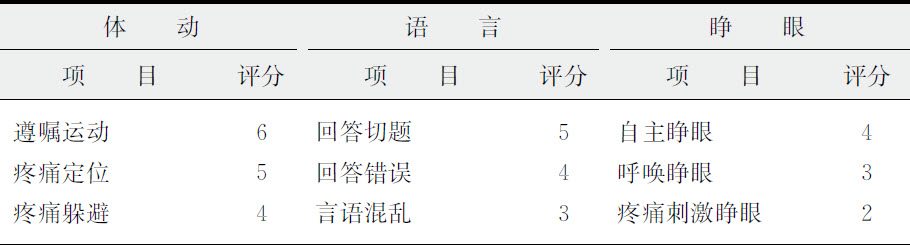
\includegraphics{./images/Image00261.jpg}
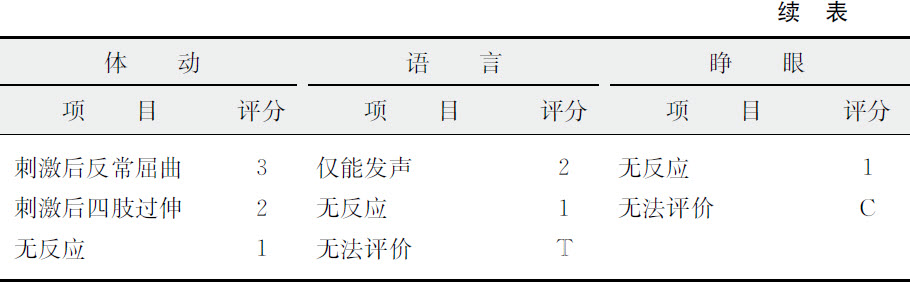
\includegraphics{./images/Image00262.jpg}
\end{table}

应用格拉斯哥昏迷评分时应注意以下细节:

(1)对患者的刺激应遵循由轻到重的原则。先呼唤、后轻拍肩膀、再推动肩膀、最后疼痛刺激,切忌一开始就给予疼痛刺激。疼痛刺激可选择叩诊锤针刺甲床、拿捏斜方肌或手指关节搔刮胸骨。

(2)所给予的疼痛刺激绝不能针对下肢,因为这时引出的体动反应可能是脊髓反射的结果,易造成混淆。

(3)呼唤患者姓名时睁眼应判断为自主睁眼。呼唤姓名不睁眼,大声嘱患者睁眼时才睁眼,判断为呼唤睁眼。

(4)判断遵嘱和语言定向力时,所提问题应尽可能简单明确,如嘱患者握手、松手,询问患者姓名、年龄,询问患者现在何处。应避免询问不易回答的复杂问题。

(5)评价时应记录观察到的最佳状态。

(6)在语言和睁眼两项中存在可能无法评价的情况。对于人工气道患者无法评价语言功能时,应记录为“人工气道”(T)。眼部直接损伤、水肿或麻痹的患者无法评价睁眼动作,应记录为“闭眼”(C)。

格拉斯哥昏迷评分的主要优点在于简便易行,主要缺点是未包括瞳孔和脑干功能的评价,而这两项内容对于脑损伤患者意识障碍的病因判断尤其重要。因此,另有一些评价工具在格拉斯哥昏迷评分的基础上,整合了脑干反射,其中以格拉斯哥-列日量表最为简便易行,临床应用也较广泛。格拉斯哥-列日量表将脑干反射定为不同分值,其余与格拉斯哥昏迷评分相同。格拉斯哥-列日量表纳入的5种脑干反射包括额-眼轮匝肌反射、垂直眼-前庭反射、瞳孔对光反射、水平眼-前庭反射和眼心反射,代表了脑干损伤自上而下不断加重,评估时应按5分到0分的顺序记录最佳状态(表\ref{tab23-2})。

\begin{table}[htbp]
\centering
\caption{格拉斯哥-列日量表(CIP)纳入的5种脑干反射}
\label{tab23-2}
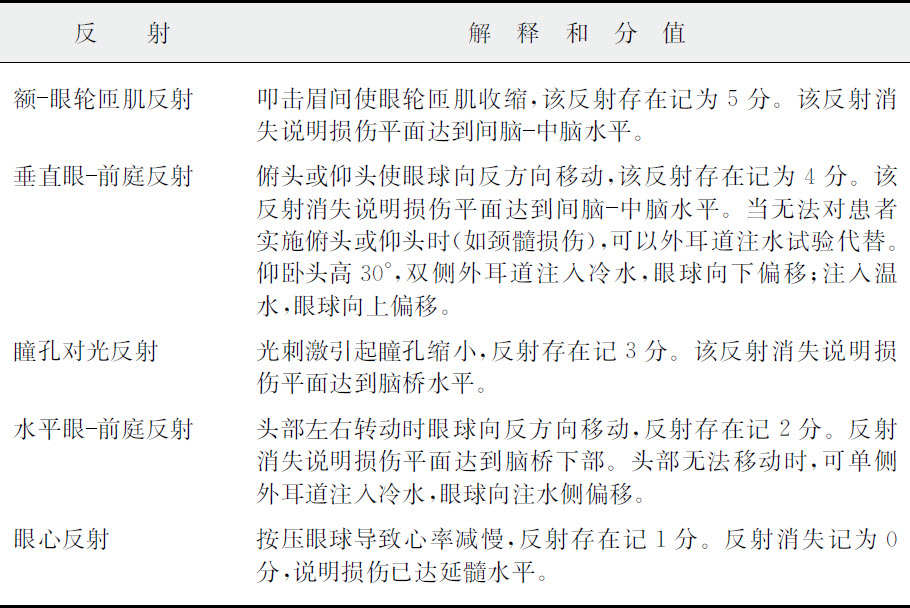
\includegraphics{./images/Image00263.jpg}
\end{table}

\subsubsection{重症医学科床旁神经系统体检应注意什么?}

体格检查在重症患者日常诊治中起着十分重要的作用。虽然重症医学科中应用的各种监测设备越来越多,但是临床医师切不可忽视基本的体格检查。体检所提供的信息也决非一两项监测参数所能代替。实施一套完整的神经系统体检需要耗时15~20分钟,并不适用于重症患者的日常巡查。通常这时采用目标式神经系统体检,即带着目的进行针对性体格检查。目标式神经系统体检应包括皮层、脑干、脑神经和肌力检查。当患者出现阳性体征时,应立即进行影像学检查,以期早期发现异常情况。

\subsubsection{颅内压监测的临床意义是什么?}

预防和治疗继发性脑损害贯穿于重症颅脑损伤患者临床救治的整个过程。现有研究表明,导致继发性脑损害的主要原因是缺血缺氧。因此,维持脑灌注是首要的治疗原则,而脑灌注压则是最直接的监测手段,临床应用也最为普遍。

脑灌注压等于平均动脉压与颅内压之间的差值,同时监测平均动脉压和颅内压,即可判断脑灌注情况。生理条件下,由于存在脑血流的自身调节机制,平均动脉压在50~150mmHg之间波动时,脑血流量维持相对恒定(图\ref{fig23-1})。脑灌注压维持在60~90mmHg可提供适宜的脑血流量。急性脑损伤患者脑血流的自身调节机制常常受到损害。在这种情况下,脑灌注压降低至60mmHg以下可能导致脑血流量的降低,引起脑缺血。脑灌注压升高至90mmHg以上,则可能导致脑血流量增加,造成血管源性脑水肿,并进一步增加颅内压。因此在临床颅内压监测中,不应仅关注颅内压,而且应综合考虑,将脑灌注压维持在适宜范围。

\begin{figure}[!htbp]
 \centering
 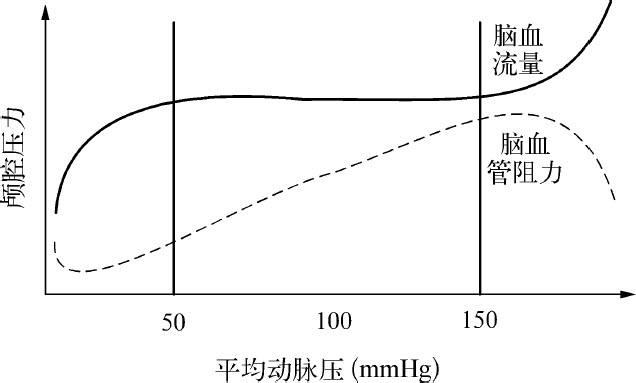
\includegraphics{./images/Image00264.jpg}
 \captionsetup{justification=centering}
 \caption{平均动脉压与脑血流量之间的关系}
 \label{fig23-1}
  \end{figure} 

颅腔为一半封闭、刚性腔隙,内容物包括脑组织、血液和脑脊液。脑组织的可压缩性很小,当颅内压升高时,血液和脑脊液被挤压出颅腔,作为代偿机制。颅内压与颅内容积之间并非线性关系(图\ref{fig23-2})。当颅内容物容积开始增加时,颅内压的升高并不明显,表现为平坦阶段,作为代偿机制的颅内血容量和脑脊液容量降低尚能发挥作用。随着颅内容积的进一步增加,代偿机制逐渐耗竭。这时即使小幅度的颅内容积增加,将导致颅内压快速升高,表现为陡峭阶段。最后,当颅内压升高到一定水平的临界压力时,曲线再次表现平坦形状,颅内压与平均动脉压几乎相等,提示颅内动脉的可扩张性达到了极限,脑灌注压几乎为0,脑动脉受到周围脑组织的压力开始闭塞。从颅内压力-容积曲线的变化趋势可见,从代偿到失代偿之间的转化是非常迅速的。在代偿阶段,临床表现可能并不明显,而一旦进入到失代偿阶段,颅内压迅速升高,脑血流灌注将在短时间内极度降低,临床常常表现出脑疝症状。这时采取处理措施,往往已经丧失了挽救脑组织的机会。因此,进行颅内压监测的另一个临床意义则在于及时发现颅内压升高的趋势,在进入失代偿期之前及时采取处理措施降低颅内压。

\begin{figure}[!htbp]
 \centering
 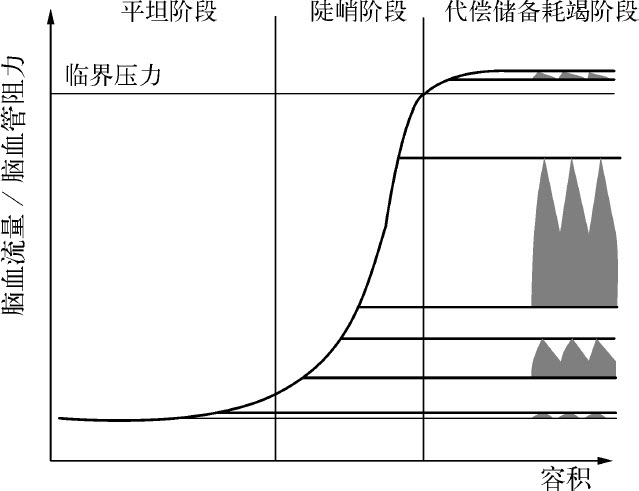
\includegraphics{./images/Image00265.jpg}
 \captionsetup{justification=centering}
 \caption{颅腔压力容积曲线}
 \label{fig23-2}
  \end{figure} 

\subsubsection{颅内压监测的主要手段和技术特点包括哪些?}

根据监测部位,颅内压监测可分为脑室内、腰大池、硬膜外、蛛网膜下腔和脑实质压力监测。根据监测原理,可分为脑脊液引流水柱传导测压和光纤-电张力测压。除此之外,还有经颅多普勒血流测定和无创颅内压监测,属于颅内压的间接测量,临床应用的准确性尚有待探讨。目前临床常用的颅内压监测技术主要是脑室穿刺置管脑脊液引流测压和光纤-电张力传感器测压,前者被认为是临床颅内压监测的“金标准”,后者则由于创伤轻微、简便易行等特点,临床应用越来越广泛。

脑室穿刺置管的位置多选择一侧侧脑室前角,脑脊液引流与测压管路连接,测压管路中充满生理盐水。水柱传导测压有赖于脑脊液的持续流出。脑水肿脑室受压常导致穿刺或监测失败。这种测压系统可反复校正零点。零点位置应是室间孔水平。依以下方法确定:外眼角与耳屏连线的中点、外眼角后1cm、翼点上方2cm处或外耳道连线中点,临床常以平卧位患者的外耳道水平作为简便定位位置。应用这种测压装置时,一定要选择非注入式压力传感器,而非普通血管内测压传感器。临床应用于血管内测压的传感器外接压力袋,当压力达到300mmHg时,每小时将有3ml液体持续注入管路系统,以防止血液回流,防止血凝块堵塞管路,颅内压的监测不宜用这种测压系统,否则将由于3ml液体的输注导致颅内压升高。颅内压监测时一定不能将肝素加入测压管路预充液体中,否则增加出血的风险,临床常规使用生理盐水作为预充液。

光纤-电张力传感器监测系统是近年来引入临床的新型颅内压监测系统。监测探头可放置到脑室、脑实质、蛛网膜下腔、硬膜外等部位。可见,该传感器扩大了颅内压监测的适应证,操作也变得相对简单。目前欧美等国家多选择这类导管进行颅内压监测。主要缺点是监测探头一旦置入,则无法重新校正零点。

\subsubsection{颅内压监测的主要并发症包括哪些?如何预防和处理?}

颅内压监测的主要并发症是感染和出血。脑实质探头的感染发生率较低。通常在颅骨钻孔处和头皮穿刺处之间建立皮下隧道,在降低感染发生率的同时,还便于固定。发生颅内感染的危险因素主要包括监测装置的置入时间超过5天和手术室外置管。置管和日常操作监测装置时应严格遵守无菌原则。常见病原菌包括金黄色葡萄球菌、表皮葡萄球菌、大肠埃希菌、克雷伯菌和链球菌。目前尚无证据表明预防性应用抗生素可降低感染发生率。

所有颅腔内置入式监测都存在导致出血的危险。与其他创伤性操作相同,恰当的培训并获得实际经验是减少出血的主要手段。患者的凝血功能状态是临床实施颅内压监测时关注的焦点。通常情况下都建议将患者的凝血功能纠正到正常范围之后再进行颅内压监测。爆发性肝衰竭患者可能合并严重的颅高压。对于这类患者,很难做到短时间内完全纠正凝血异常。虽然近期有研究显示肝移植患者在应用脑实质颅内压监测时的安全性,但多数单位仍然倾向于为肝衰竭患者选择硬膜外或蛛网膜下腔探头进行颅内压监测。

\subsubsection{脑代谢监测的临床意义是什么?临床可利用的床旁脑代谢监测手段包括哪些?}

大脑具有极高的代谢率。虽然脑的重量只占体重的2%,但静息脑血流量却占到心输出量的15%,氧耗量是全身的20%。因此,大脑需要持续稳定的血流灌注,当存在缺氧或灌注不足时,将发生一系列生物化学反应的异常。脑代谢监测的目的就是尽早发现这些异常情况。

目前可利用的床旁脑代谢监测分为两类,脑氧监测和脑组织微透析监测。前者包括多种监测技术,其中临床最常应用的是颈静脉血氧饱和度监测,其他还有近红外光谱仪经颅脑氧饱和度监测和脑组织氧分压监测。近年来,脑组织氧分压和脑组织微透析监测的临床应用越来越多,代表了脑代谢监测的主要进展
\protect\hyperlink{text00029.htmlux5cux23ch3-28}{\textsuperscript{{[}3{]}}}
\textsuperscript{~}
\protect\hyperlink{text00029.htmlux5cux23ch6-28}{\textsuperscript{{[}6{]}}}
。

\subsubsection{颈静脉血氧饱和度监测的原理是什么?}

颈静脉血氧饱和度反映脑组织中未被利用的氧。监测颈静脉血氧饱和度可反映脑氧供给和消耗之间的平衡,并间接反映脑血流灌注。颈静脉血氧饱和度监测部位应选择颈静脉球部,目的在于避免头皮静脉和面静脉血液的掺杂。

脑氧耗量(CMRO\textsubscript{2}
)等于单位时间内进入和流出大脑的氧量之差:

\begin{center}
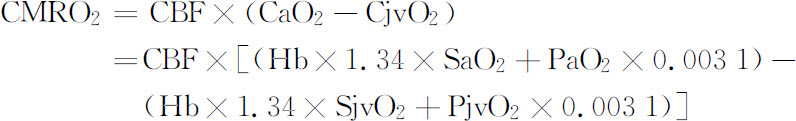
\includegraphics{./images/Image00266.jpg}
\end{center}

公式中CaO\textsubscript{2} 、SaO\textsubscript{2} 和PaO\textsubscript{2}
分别为动脉血氧含量、氧饱和度和氧分压;CjvO\textsubscript{2}
、SjvO\textsubscript{2} 和PjvO\textsubscript{2}
分别为颈静脉血氧含量、氧饱和度和氧分压;Hb为血红蛋白浓度,CBF为脑血流量。

血液中物理溶解的氧量很少,可忽略不计。公式表示为:

\begin{center}

\includegraphics{./images/Image00267.jpg}
\end{center}

公式可变形为: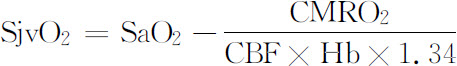
\includegraphics{./images/Image00268.jpg}

可简化为:
\includegraphics{./images/Image00269.jpg}

由该公式可见,SjvO\textsubscript{2}
由动脉血氧饱和度、脑氧耗量、脑血流量和血红蛋白浓度共同决定。临床实际中,血红蛋白浓度一般不会在短时间内发生剧烈变化,公式可再次简化为:
\includegraphics{./images/Image00270.jpg}

正常情况下,当脑氧耗量升高时,脑血流量随之升高;脑血流量降低时,脑氧耗量也随之降低,称为脑代谢-血流耦联。这时颈静脉血氧饱和度维持不变,脑氧提取率也维持不变。病理情况下,脑代谢-血流耦联受损,将导致脑氧提取的变化,表现为颈静脉血氧饱和度降低或升高。颈静脉血氧饱和度监测的主要目的也就是尽早发现脑血流与脑代谢之间的平衡失调。

\subsubsection{颈静脉血氧饱和度升高和降低的临床意义是什么?}

健康人采样显示,颈静脉血氧饱和度(SjvO\textsubscript{2}
)的正常范围在55%~71%之间,平均62%。队列研究提示,颈静脉血氧饱和度低于50%,脑损伤患者的死亡率增加1倍。对接受心血管手术的患者,颈静脉血氧饱和度低于50%将导致术后神经系统并发症的发生率明显增多。对于脑损伤患者合适的颈静脉血氧饱和度水平,目前尚缺乏明确的推荐意见,多数选择55%~75%为颈静脉血氧饱和度的目标界限。

表\ref{tab23-3}显示了导致颈静脉血氧饱和度降低和升高的主要因素。

表\ref{tab23-3} 导致颈静脉血氧饱和度(SjvO\textsubscript{2}
)降低和升高的主要因素

\begin{center}

\includegraphics{./images/Image00271.jpg}
\end{center}

\subsubsection{如何确定颈静脉血氧饱和度监测导管放置的深度?}

颈内静脉逆向置管的标准方法是在环状软骨水平,沿胸锁乳突肌锁骨头内侧,针尖指向头部穿刺置管。置管成功后导管放置深度是影响监测结果的关键问题。颈内静脉出颅后还汇集面静脉血流,因此应将导管尖端置入颈静脉球部(图\ref{fig23-3}),此处约仅掺杂3%的面静脉血流。放置时应将导管尖端尽量靠近颈静脉球部顶端,导管后撤2cm将使面静脉血流掺杂升高到10%。临床测量时可应用乳突作为颈静脉球部的体表标志。但是放置导管后应常规进行X线摄片定位。颈部侧位片要求导管尖端超过第1~2颈椎,并尽可能靠近颅底。在后前位片,导管尖端应超过寰枕关节与眶底连线,并超过双侧乳突连线。

\begin{figure}[!htbp]
 \centering
 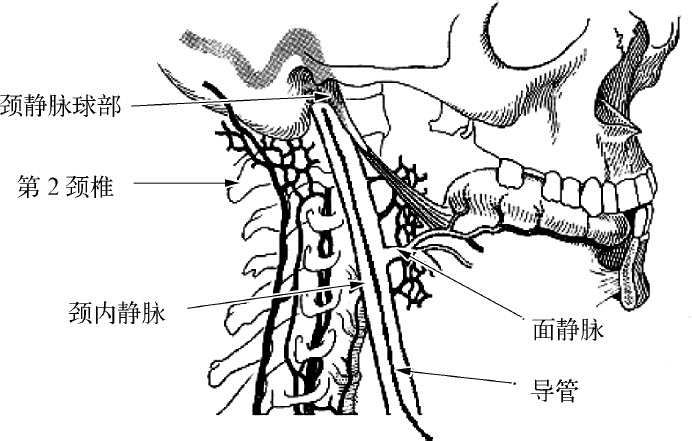
\includegraphics{./images/Image00272.jpg}
 \captionsetup{justification=centering}
 \caption{颈静脉球部解剖示意图}
 \label{fig23-3}
  \end{figure} 

\subsubsection{应选择哪一侧进行颈静脉血氧饱和度监测?}

从测定原理可见,颈静脉血氧饱和度反映全脑氧代谢情况,因此,左右颈静脉氧饱和度的一致性会影响到监测结果的准确性。尸体解剖发现,皮层下区域的静脉多回流至左侧静脉窦,而皮层区域多回流至右侧。目前倾向于选择优势侧颈静脉作为监测部位。临床确定方法有3种:①实施颅内压监测的患者,交替按压双侧颈静脉,颅内压升高幅度较大的一侧为优势侧;②观察CT显示的颈静脉孔,较大的一侧为优势侧;③超声扫描血流量较多的一侧为优势侧。当缺乏这些确定方法时,由于大多数个体的右侧静脉窦较大,可首先选择右侧作为监测部位。有些研究建议选择病变侧作为监测部位,但目前尚存在争论。

\subsubsection{近红外光谱仪经颅脑氧饱和度监测的优点和缺点是什么?}

光线穿过色基时被散射和吸收,光线衰减的程度与色基的浓度相关。波长为700~1000nm的近红外光具有良好的组织穿透力,且其衰减程度与血红蛋白中的铁及细胞色素a3中的铜含量成正比。氧合血红蛋白与去氧血红蛋白的光吸收波长不同,由此可计算出组织氧饱和度。近红外光谱仪即利用这一原理进行脑氧饱和度测定,其优点在于无创和连续监测。然而,与脉搏血氧饱和度不同,近红外光谱仪测定的脑氧饱和度不能区分动、静脉血,所监测的是整个脑组织血管床的氧饱和度,包括动脉、静脉和毛细血管,其中约70%的成分来自静脉血。此外,由于很难排除颅外组织对光线的吸收和散射,也使近红外光谱测定结果的可靠性受到置疑。总的来看,作为床旁脑氧监测手段,近红外光谱仪技术仍需要进一步探索。

\subsubsection{脑组织氧分压监测技术主要包括哪些?}

目前临床中常用的商品化脑组织氧分压监测技术主要有两种,Licox(Integra
Neuroscience,Plainsboro,NJ)和Neurotrend(Diametrics
Medical,St.Paul,MN)系统,两种方法的监测技术不同。Licox系统采用Clark氧电极,仅监测氧分压;而Neurotrend系统应用荧光光纤传感器,可同时监测氧分压、二氧化碳分压和pH值。另有其他监测系统,但应用应用较少,如Neurovent-PTemp\textsuperscript{®}
(Raumedic AG,Munchberg,Germany)和OxyLab pO\textsubscript{2}
\textsuperscript{®} (Oxford Optronix Ltd.,Oxford,UK)。

\subsubsection{Clark氧电极脑组织氧分压监测的原理是什么?}

Clark氧电极由一层覆盖电解质的膜和两个金属电极组成,利用贵金属的电化学特性测定组织中的氧分压。氧通过膜弥散到阴极衰减。氧分压越高,跨膜弥散量越多。参考电极与监测电极之间电压差与氧分子在阴极的衰减成正比。这一过程与温度相关,因此脑组织氧分压探头需同时整合温度传感器。脑组织温度每变化1℃,脑代谢变化5%~13%,从而影响到脑血流量和颅内压。

\subsubsection{脑组织氧分压监测结果的临床意义是什么?}

近期研究提示,脑组织氧分压与脑血流量和监测局部脑动静脉氧含量差呈明显正相关。现有资料表明,脑组织氧分压并非只是简单地反映脑缺血缺氧,更可能是代表了局部脑组织氧供给和细胞氧消耗之间的平衡。同时,脑组织氧分压监测还受到氧在毛细血管和脑细胞间弥散距离、探头放置区域局部脑组织中小动脉和小静脉分布比例的影响。总体考虑,脑组织氧分压反映的是氧在局部脑组织的弥散和贮存量,其中脑血流量与脑动-静脉血氧含量差的乘积,反映的是从动脉血向脑组织弥散的氧量。

\subsubsection{如何确定脑组织氧分压监测探头的放置位置?}

与颈静脉血氧饱和度不同,脑组织氧分压监测的是局部脑组织氧合状况。因此,监测探头的放置位置将对监测结果产生明显影响。通常选择放置于病变侧的额叶。对于弥漫性脑肿胀或轴索损伤的患者,常选择右侧额叶。对于蛛网膜下腔出血患者,常放置在动脉瘤破裂的同侧,或出血厚度较大的一侧,目的在于通过监测早期发现脑血管痉挛。应避免将脑组织氧分压监测探头置于已经梗死的脑组织或血肿腔内。在监测装置置入前后行影像学检查,以确定探头位置。脑组织氧分压监测操作指南推荐,监测探头放置到位后,应提高吸入氧浓度,观察监测参数的变化,以确定监测的确切性。

\subsubsection{提示脑缺血的脑组织氧分压监测界值是多少?临床意义是什么?}

生理学研究显示,线粒体氧分压必须维持在1.5mmHg以上才能正常产生三磷酸腺苷,与这种氧分压水平相对应的脑组织氧分压为15~20mmHg。多项针对脑损伤患者的队列研究表明,脑组织氧分压低于15~20mmHg的次数、持续时间和幅度是不良神经系统转归的独立危险因素。

临床应用脑组织氧分压监测的主要目的在于及早发现脑组织低灌注,并指导治疗。长期以来,临床依照颅内压或脑灌注压指导脑损伤患者的救治,形成脑灌注目标式救治策略。然而流行病学研究显示,重度脑创伤患者急性期,颅内压和脑灌注压维持于正常水平时,也有将近半数患者表现为短暂或持续脑组织氧分压降低。近年来,临床中将常用的颅内压监测与脑组织氧分压监测整合,形成脑氧合目标式救治流程。回顾性对照研究显示,整合脑组织氧分压监测与单独颅内压/脑灌注压监测相比,死亡率降低,神经系统转归改善。然而,目前尚缺乏相应的高级别临床研究证据。

\subsubsection{脑组织微透析监测的技术原理是什么?}

脑组织微透析监测是将管壁材料为聚酰胺微透析膜的纤细导管置入脑组织中,内充透析液。脑细胞外液中小于微透析膜孔径的物质可顺浓度梯度弥散到透析液中。定时收集透析液进行生化分析,可监测脑组织细胞外液的代谢改变。透析液多采用生理盐水。微透析导管具有不同规格的半透膜孔径。孔径越大,生物大分子(如细胞因子)透过半透膜的可能性越大,越有利于减轻细胞因子对细胞损伤和炎症反应的作用。目前已经拥有2万、10万和300万道尔顿孔径的监测导管。

\subsubsection{通过脑组织微透析监测可获得哪些信息?}

理论上,凡是可透过微透析膜的物质均可进行监测。表\ref{tab23-4}列出了目前临床主要监测的4类参数。

\begin{table}[htbp]
\centering
\caption{脑组织微透析监测的主要参数}
\label{tab23-4}
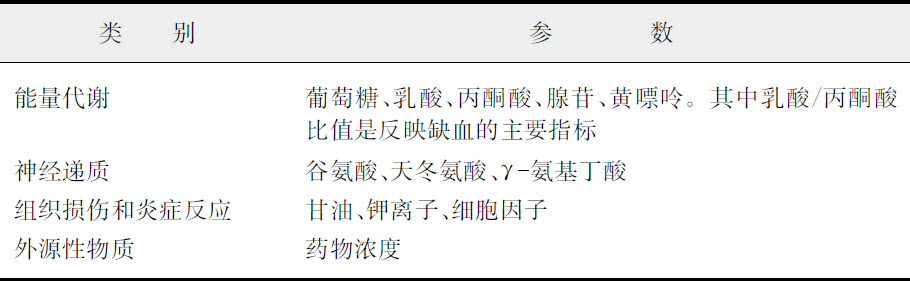
\includegraphics{./images/Image00273.jpg}
\end{table}

\subsubsection{反映脑缺血的微透析监测参数主要包括哪些?临床意义是什么?}

葡萄糖为细胞代谢的能量底物,氧则是细胞进行能量代谢所必需。有氧条件下,每分子葡萄糖代谢生产38分子三磷酸腺苷(ATP),而糖的无氧酵解仅生成2分子三磷酸腺苷。脑的能量储备很低,因此依赖于持续的血液供应以提供氧和能量代谢底物。缺氧缺血时,能量储备在短时间内耗竭,从而造成一系列病理生理学损害。组织的代谢监测反映组织供血供氧情况,以期在出现生化异常的早期给予积极处理。现有资料表明,反映脑缺血的微透析监测敏感指标是乳酸/丙酮酸比值和葡萄糖浓度,预警界限分别为>30和<0.8mmol/L。

\subsubsection{如何确定微透析监测导管的放置部位?}

微透析属局部监测,导管位置影响监测参数的判读。有研究针对重度脑创伤患者进行了包括微透析在内的多种脑功能监测。微透析和脑组织氧分压探头放置于损伤脑组织周围,结果显示术后损伤局部脑梗死的患者,脑组织氧分压明显降低,微透析监测乳酸水平明显升高。2004年发表的专家共识推荐对于弥漫性脑损伤患者,探头应放置于右侧额叶;局灶性脑损伤患者,应在损伤部位周围实施微透析监测,有条件时,可在非损伤区放置第二个监测探头。

\subsection{脑功能保护和支持}

\subsubsection{重症脑损伤患者的气道管理有哪些特点?}

重症脑损伤患者是呼吸系统并发症的高危群体,危险因素包括意识障碍、气道保护性反射异常、气道机械性梗阻以及中枢性呼吸肌无力。对这些患者采取及时有效的气道管理,是改善转归的重要决定因素。

脑损伤患者的中枢神经系统对缺血缺氧的耐受性明显降低,一旦发生异常情况,处理不及时将导致灾难性后果。这类患者建立人工气道的适应证应适当放宽。脑损伤患者行紧急气管插管的适应证包括:①意识障碍,格拉斯哥昏迷评分低于9分;②咽喉部保护性反射丧失;③呼吸节律不规则,有较长时间的呼吸暂停;④未被控制的癫痫持续状态;⑤其他需要机械通气支持的氧合和(或)通气功能障碍。

尤其要强调的是,脑损伤患者行气管插管时需应用镇痛镇静剂避免颅内压升高。镇静剂的选择原则是起效迅速,对中枢神经系统无附加损害。阿片类药物对循环的影响较小,并有特效拮抗剂纳络酮;苯二氮䓬
类药物中,咪唑安定起效快,对心血管系统的影响也较轻,是理想的镇痛镇静药物。异丙酚为新型快速、短效、强效静脉麻醉药,但是对循环的影响较大,如导致平均动脉压降低,可能导致脑灌注压降低,应用时需慎重。镇痛镇静药的选择应基于患者当时的循环状况,以及对气管插管困难程度的判断。插管途径首选经口插管,对于颅底损伤、脑脊液漏和经蝶胺手术患者,禁忌行经鼻气管插管。

对于保留人工气道的患者,应严格掌握拔管指征。拔管前,必须仔细判断患者的吞咽和咳嗽反射。呼吸道的正常反射有赖于第V、VII、IX、X和XII对脑神经的正常功能。这些脑神经损伤可发生吞咽功能、舌体运动和声带功能异常,导致上呼吸道梗阻,严重时发生肺水肿。表\ref{tab23-5}列出了拔除气管插管的判断指标和操作顺序。最后判断的指标为刺激支气管隆突时的咳嗽反射,若咳嗽反射存在,提示存在气道自洁能力,有利于拔管后痰液引流和感染控制。切忌反复试验,以免引起患者剧烈咳嗽,导致血压升高,增加脑出血和脑水肿的危险。

\begin{table}[htbp]
\centering
\caption{重症颅脑损伤患者拔除气管插管的步骤}
\label{tab23-5}
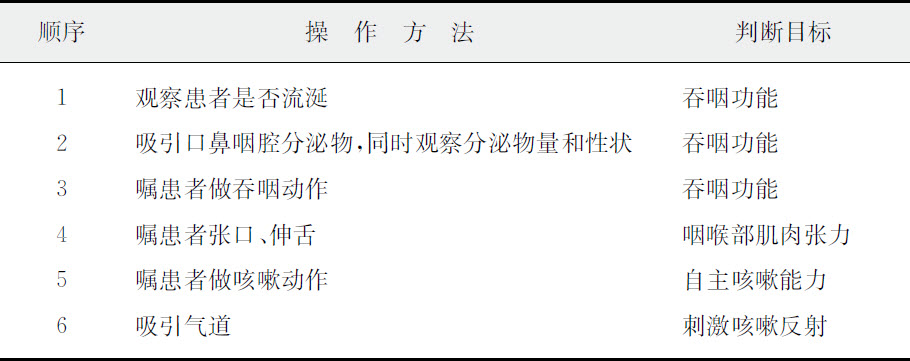
\includegraphics{./images/Image00275.jpg}
\end{table}

脑损伤患者行气管切开的时机,仍是目前存在争论的问题。虽然气管切开置管有利于气道维护,患者耐受性提高,有利于减少死腔、痰液引流和呼吸做功等,但是现有资料并未证实早期气管切开能改善患者转归和预后。大样本随机对照研究比较了重症患者机械通气后早期(6~8天)和晚期(13~15天)接受气管切开,虽然早期组呼吸机相关性肺炎的发生率有降低的趋势,但未获得统计学意义,两组患者死亡率和住院时间也无显著性差异。对于脑损伤患者,考虑到专科特征性,根据有限的证据,推荐当存在以下情况时,早期行气管切开------①脑损伤1周后格拉斯哥昏迷评分仍然低于9分;②脑干损伤;③神经肌肉疾患;④预计短期内无法撤离机械通气。

\subsubsection{临床实施过度通气应注意什么?}

对于脑血管二氧化碳反应性保留完好的患者,过度通气诱发的低碳酸血症可导致急性脑血管收缩,颅内血容量降低,颅内压降低。急性低碳酸血症早期,脑血流和压力自身调节曲线右移,表现为在较高平均动脉压条件下维持较低的脑血流量和颅内压。随着碳酸酐酶和其他非碳酸氢盐缓冲系统的参与,自身调节机制逐渐适应,脑血管丧失了对低碳酸血症的收缩反应,曲线重新左移,导致在低二氧化碳分压水平下脑血流量恢复。多数患者在3~4小时内重新建立新的稳态。针对脑损伤患者的研究显示,低碳酸血症降低颅内压的作用一般都会在6~12小时后消失。

由于过度低碳酸血症引起脑血管过度收缩,将导致局部或广泛性脑缺血,因此不建议预防性应用过度通气,而仅是作为实施其他更有效或更持久的降低颅内压措施前的一种暂时性紧急辅助手段。脑损伤患者动脉血二氧化碳分压的理想水平为35~40mmHg。对于持续颅高压患者,当脱水剂、脑室引流、镇静肌松剂等治疗无效时,可选择实施过度通气治疗,但建议进行脑氧代谢监测。患者颅内压对过度通气无明显反应,通常提示预后不良。

临床处理中另一个需要注意的问题是过度通气的撤除。动脉血二氧化碳分压从低水平快速恢复到基础水平,可造成脑血管扩张,导致脑血容量增加,出现颅内压反跳。因此,当撤除过度通气时,应逐渐增加通气量,使二氧化碳分压逐渐恢复到正常水平。

另一方面,由于通气不足,动脉血二氧化碳分压升高,导致脑血管扩张,脑血容量增加,颅压升高。因此,高颅压患者进行机械通气支持时,应密切监测动脉血二氧化碳分压,避免高碳酸血症的发生。

\subsubsection{脑损伤患者应用呼气末正压时应注意什么?}

呼气末正压(PEEP)通过多种机制影响颅内压。由于胸腔和颅腔解剖位置的毗邻关系,应用PEEP时,胸腔内压力的升高可直接经过颈部传导至颅腔。应用PEEP使患者气道峰压和气道平均压升高,颈静脉回流受阻,颅内血容量和脑脊液量增加,颅内压升高。此外,应用PEEP后导致心输出量和平均动脉压降低时,由于脑血流灌注的下降会导致脑血管反射性扩张,也可能导致颅内压升高
\protect\hyperlink{text00029.htmlux5cux23ch7-28}{\textsuperscript{{[}7{]}}}
。

PEEP对颅内压的作用,受到多种因素影响,主要包括颅腔顺应性、呼吸系统顺应性和基础颅内压水平。对于颅腔顺应性降低的患者,PEEP升高颅内压的作用更为明显。呼吸系统顺应性也参与影响颅内压的幅度:胸廓顺应性降低,PEEP对颅内压的作用增强;肺顺应性降低,PEEP对颅内压的作用减弱。对于颅内压已经明显升高的患者,应用PEEP后颅内压进一步升高的幅度减小。一般来说,临床应用15cm
H\textsubscript{2}
O以下的PEEP,不会对患者的颅内压造成明显影响。当临床需要应用高水平PEEP,或患者存在颅内压升高的危险因素时,应严密监测颅内压。

\subsubsection{脑损伤患者容量管理的目标是什么?应用渗透性利尿剂时应注意什么?}

脑损伤患者容量管理的目标是维持组织灌注前提下的限制性液体管理。早期限制液体入量、“使患者处于脱水状态”的观念已被证实是错误的。限制液体入量造成的低血容量状态可导致脑灌注压降低,加重脑组织缺血缺氧,且没有证据显示,限制液体可以改善脑水肿。维持正常的血容量、避免出现脑低灌注,对颅内压是无害的。同时,应及时纠正血浆的低渗状态(渗透压低于280mOsm/kg),研究显示,维持轻微高渗状态(血浆渗透压300~315mOsm/kg)有利于减少脑细胞内水分,减轻脑水肿
\protect\hyperlink{text00029.htmlux5cux23ch8-28}{\textsuperscript{{[}8{]}}}
。血浆渗透压依以下公式计算:

\begin{center}

\includegraphics{./images/Image00276.jpg}
\end{center}

其中BUN为尿素氮,血浆渗透压的正常值为280~290mOsm/kg。

渗透性利尿剂治疗可维持血浆高渗状态,主要包括甘露醇和高张盐水。常用甘露醇0.25~1.0g/kg静脉注射,每4~6小时一次。在达到获得预期疗效的最低渗透浓度同时,需监测渗透压间隙,即:

渗透压间隙=测定的渗透压-计算渗透压(正常值≤10mOsm/kg)

应用甘露醇的治疗目标是使渗透压间隙达到或超过15mOsm/kg。但血浆渗透压不宜超过320mOsm/kg,研究显示并不会取得更好的疗效,反而使渗透压间隙进一步增加,导致急性肾衰竭。

高张盐水可通过提高血浆钠水平升高血浆渗透压。应用高张盐水溶液时,需要监测血清钠水平,以避免血钠浓度变化过快。高张盐水溶液可能导致或加重充血性心力衰竭,因此高危患者慎用。应用3%氯化钠溶液时,可每4~6小时静脉注射150ml,或以每小时0.5~1.0ml/kg的速度持续静脉注射。7.5%氯化钠溶液2ml/kg的剂量静脉注射,每6小时一次。

当血浆渗透压高于正常水平超过48小时后,将产生细胞内渗透颗粒,细胞内容量达到新的平衡。此后若迅速纠正血浆渗透压将导致自由水进入颅内间隙。因此,一旦开始应用长效的渗透性药物后,必须逐渐减量,以便自发性渗透分子排出。这一原则适用于各种渗透性药物。

\subsubsection{脑损伤患者血压控制目标是多少?}

不同类型的脑损伤患者,由于损伤机制和颅内血流动力学特点不同,具有不同的血压控制目标。

对于颅脑创伤患者,脑灌注压一直是临床关注的焦点,将脑灌注压维持于70mmHg以上,也一直是临床处理颅脑创伤患者的标准。随着临床颅内压监测技术应用的普及和脑灌注区目标管理研究的开展,对颅脑创伤患者脑灌注区目标界值也提出了质疑。虽然尚缺乏高级别循证医学证据支持,2007年美国神经外科医师协会发表的临床指南推荐,对于重度颅脑创伤患者,由于存在导致ARDS的危险,应避免大量补液和应用升压药物将脑灌注压维持在高于70mmHg的水平,同时也要避免脑灌注压低于50mmHg。因此,这类患者的脑灌注压控制目标是在50~70mmHg的范围内。脑血流自身调节能力尚存的患者,通常可耐受较高的脑灌注压。有条件时,应监测患者的脑血流和代谢状况。

对于自发性脑出血患者,2007年美国卒中学会推荐的血压控制方案包括:

(1)当动脉收缩压高于200mmHg或平均动脉压高于150mmHg时,应以持续静脉给药的方式积极降低血压,并每5分钟监测血压一次;

(2)当动脉收缩压高于180mmHg或平均动脉压高于130mmHg时,若有证据或怀疑颅内压升高,应进行颅内压监测,并将脑灌注压维持在高于60~80mmHg的水平;

(3)当动脉收缩压高于180mmHg或平均动脉压高于130mmHg,但无颅内压升高,应以间断或持续静脉给药的方式缓慢降低血压,目标为平均动脉压110mmHg或160/90mmHg,并每15分钟监测血压一次。

对缺血性脑卒中患者的血压控制,目前还存在争议。多数患者会在卒中发生后24小时内出现自发性血压下降。总的来说,除非患者具有需要紧急降低血压的其他适应证,对这类患者的降压治疗应持谨慎态度。对具有重组组织型纤溶酶原激活剂治疗适应证的患者,在溶栓前应将血压控制在185/110mmHg以下,并维持该血压水平直至重组组织型纤溶酶原激活剂治疗后24小时。该原则适用于接受其他血管再通治疗的患者,如动脉内介入溶栓。对于无法实施溶栓的患者,或患者接受溶栓治疗超过24小时,现有共识推荐的高血压处理界值为220/120mmHg
\protect\hyperlink{text00029.htmlux5cux23ch9-28}{\textsuperscript{{[}9{]}}}
\textsuperscript{,}
\protect\hyperlink{text00029.htmlux5cux23ch10-28}{\textsuperscript{{[}10{]}}}
。目前正在进行缺血性脑卒中患者急性期血压控制对转归影响的相关研究,在新的研究结果发表前,上述高血压处理界值,仍然是临床参照的标准。

对于动脉瘤破裂导致蛛网膜下腔出血患者,由于脑血管痉挛造成的迟发性脑缺血,一直是临床处理的难点问题。临床也曾出现以高血容量、高血压和血液稀释为代表的3H治疗策略。2011年,美国神经重症学会发表了蛛网膜下腔出血临床处理指南,其中对患者的循环支持,提出了相应的推荐意见
\protect\hyperlink{text00029.htmlux5cux23ch11-28}{\textsuperscript{{[}11{]}}}
。尼莫地平具有预防脑血管痉挛的作用,口服60mg、每4小时一次,疗程21天。若患者出现血压降低,可减小剂量,缩短用药间隔。对于不能耐受的患者,应停止使用。蛛网膜下腔出血患者容量支持目标是正常血容量,不推荐诱导性高血容量。对于临床怀疑迟发性脑缺血的患者,可进行诱导性高血压试验。应用升压药物逐步提高患者血压,并进行神经系统体检,以确定最佳血压水平。对于升压治疗仍不能缓解脑缺血症状的患者,可应用正性肌力药物。使用β\textsubscript{2}
受体激动剂------如多巴酚丁胺,可能会导致平均动脉压降低,这时应增加升压药剂量。除非患者存在红细胞增多症,不推荐应用血液稀释治疗。

\subsubsection{如何评价低温治疗的脑保护作用?低温治疗的临床实施应注意哪些问题?}

现有资料表明,低温治疗可改善心跳骤停后全脑缺血性损害患者的远期神经系统功能转归。但是对于局灶性脑损伤患者,如颅脑创伤、缺血性卒中和脑出血,并未获得循证医学证据支持。由于存在严重的副作用,现对低温治疗多持谨慎态度。然而,对于常规内科治疗无效的重度颅高压患者,低温又往往成为临床治疗时不得不选择的控制颅高压的方法
\protect\hyperlink{text00029.htmlux5cux23ch12-28}{\textsuperscript{{[}12{]}}}
。

临床实施低温治疗时应注意的问题主要包括:

(1)通常将目标体温控制在33~35℃(中心体温,如膀胱温度或血温)。

(2)疗程为24~48小时。目前无研究探讨长时间低温治疗的效果。低温治疗需要注意的是,应严格控制复温速度,过快的复温将导致颅内压反跳性升高。文献报道的复温方法多为被动复温。若进行颅内压监测,可根据颅内压的变化控制复温速度。

(3)由于多数患者在低温过程中发生寒战,推荐应用镇静剂和肌松剂。目前镇静剂多选择咪达唑仑和异丙酚,部分研究同时应用芬太尼。综合低温治疗的文献报道,联合应用肌松剂的情况超过80%。

(4)低温治疗的并发症主要包括心律失常、电解质紊乱、凝血功能异常和感染,治疗过程中应密切监测,降低发生并发症的危险。

(5)现有资料表明,单纯头部降温不能获得确切的临床效果。

\subsubsection{何为脑损伤的程序化治疗?}

重型颅脑损伤属多因素影响的危重症,目前尚缺乏单一有效的治疗手段,临床治疗中多采用程序化救治策略,也可称之为集束化治疗。这种治疗策略包括两个特点,首先是设定治疗目标,现在多选择颅内压或脑灌注压为治疗目标,部分研究整合了脑氧监测目标;其次是将治疗手段由简单到复杂分成不同级别,对照治疗目标判断是否达到分级实施。表\ref{tab23-6}列出了目前采用较多的针对颅脑创伤的治疗措施分级。可以发现一线治疗包括针对所有危重患者均需实施的处理措施,当这些措施不能达到治疗目的时,启动下一级治疗。图\ref{fig23-4}以流程图的形式列举了以颅内压作为目标的重度颅脑创伤的程序化治疗
\protect\hyperlink{text00029.htmlux5cux23ch13-28}{\textsuperscript{{[}13{]}}}
。

\begin{table}[htbp]
\centering
\caption{颅脑创伤的治疗措施分级}
\label{tab23-6}
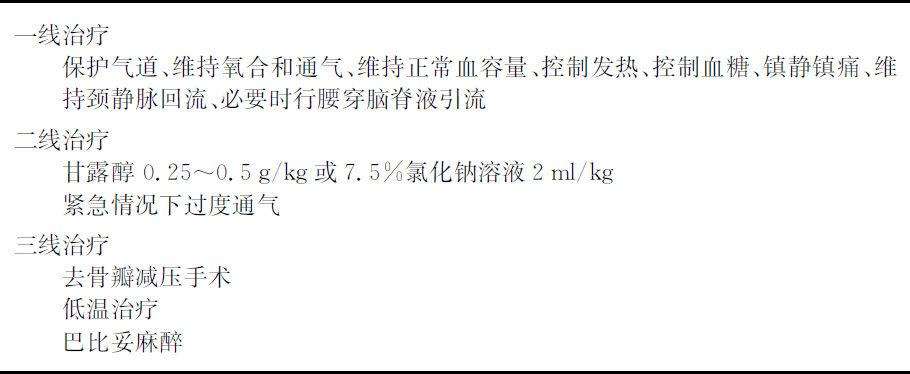
\includegraphics{./images/Image00277.jpg}
\end{table}

\begin{figure}[!htbp]
 \centering
 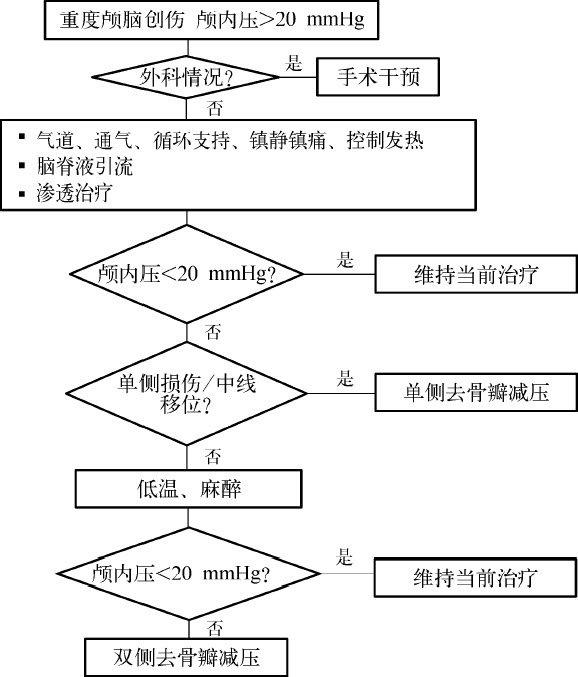
\includegraphics[width=\textwidth,height=\textheight,keepaspectratio]{./images/Image00278.jpg}
 \captionsetup{justification=centering}
 \caption{重度颅脑创伤的程序化治疗流程}
 \label{fig23-4}
  \end{figure} 

\begin{center}\rule{0.5\linewidth}{\linethickness}\end{center}

参考文献

\protect\hyperlink{text00029.htmlux5cux23ch1-28-back}{{[}1{]}} .Cooper
DJ,Rosenfeld JV,Murray L,et al.Decompressive craniectomy in diffuse
traumatic brain injury.N Engl J Med,2011,364(16):1493-1502.

\protect\hyperlink{text00029.htmlux5cux23ch2-28-back}{{[}2{]}} .Clifton
GL,Valadka A,Zygun D,et al.Very early hypothermia induction in
patients with severe brain injury(the National Acute Brain Injury
Study:Hypothermia II):a randomized trial.Lancet
Neurol,2011,10(2):131-139.

\protect\hyperlink{text00029.htmlux5cux23ch3-28-back}{{[}3{]}}
.刘大为.实用重症医学.北京:人民卫生出版社,2010,155-167,758-765.

{[}4{]}.Messerer M,Daniel RT,Oddo M.Neuromonitoring after major
neurosurgical procedures.Minerva Anestesiol,2012,78(7):810-822.

{[}5{]}.Rao GSU,Durga P.Changing trends in monitoring brain
ischemia:from intracranial pressure to cerebral oximetry.Curr Opin
Anaesthesiol,2011,24(5):487-494.

\protect\hyperlink{text00029.htmlux5cux23ch6-28-back}{{[}6{]}}
.Hillered L,Persson L,Nilsson P,et al.Continuous monitoring of
cerebral metabolism in traumatic brain injury:a focus on cerebral
microdialysis.Curr Opin Crit Care,2006,12(2):112-118.

\protect\hyperlink{text00029.htmlux5cux23ch7-28-back}{{[}7{]}} .Nyquist
P,Stevens RD,Mirski MA.Neurologic Injury and Mechanical
Ventilation.Neurocrit Care,2008,9(3):400-408.

\protect\hyperlink{text00029.htmlux5cux23ch8-28-back}{{[}8{]}}
.Guidelines for the management of severe traumatic brain injury.J
Neurotrauma,2007,24(Sl):1-106.

\protect\hyperlink{text00029.htmlux5cux23ch9-28-back}{{[}9{]}}
.Broderick J,Connolly S,Feldmann E,et al.Guidelines for the
management of spontaneous intracerebral hemorrhage in adults:2007
update:a guideline from the American Heart Association/American Stroke
Association Stroke Council,High Blood Pressure Research Council,and
the Quality of Care and Outcomes in Research Interdisciplinary Working
Group.Stroke,2007,38(6):2001-2023.

\protect\hyperlink{text00029.htmlux5cux23ch10-28-back}{{[}10{]}} .Adams
HP,Jr.,del Zoppo G,Alberts MJ,et al.Guidelines for the early
management of adults with ischemic stroke:a guideline from the American
Heart Association/American Stroke Association Stroke Council,Clinical
Cardiology Council,Cardiovascular Radiology and Intervention
Council,and the Atherosclerotic Peripheral Vascular Disease and Quality
of Care Outcomes in Research Interdisciplinary Working Groups:the
American Academy of Neurology affirms the value of this guideline as an
educational tool for neurologists.Stroke,2007,38(5):1655-1711.

\protect\hyperlink{text00029.htmlux5cux23ch11-28-back}{{[}11{]}}
.Diringer MN,Bleck TP,Hemphill JC,et al.Critical care management of
patients following aneurysmal subarachnoid hemorrhage:recommendations
from the Neurocritical Care Society's Multidisciplinary Consensus
Conference.Neurocrit Care,2011,15(2):211-240.

\protect\hyperlink{text00029.htmlux5cux23ch12-28-back}{{[}12{]}}
.Polderman KH.Induced hypothermia and fever control for prevention and
treatment of neurological injuries.Lancet,2008,371:1955-1969.

\protect\hyperlink{text00029.htmlux5cux23ch13-28-back}{{[}13{]}}
.Vincent JL,Berre J.Primer on medical management of severe brain
injury.Crit Care Med,2005,33(6):1392-1399.

\protect\hypertarget{text00030.html}{}{}

